\chapter{Comparación de resultados}
\label{cap:comp}

\section{Tasa de éxito y tiempo (experimento A)}
La tabla~\ref{tab:resumenA} resume las \ejecA{} corridas del experimento A. El resultado más
claro es que solo tres algoritmos encontraron ciclos:
\begin{itemize}
  \item \alg{ABC}: \exitosAABC{} corridas exitosas, en \resueltasAABC{} grafos distintos.
  \item \alg{ACO + Pósa}: \exitosAACOposa{} corridas exitosas, también en \resueltasAACOposa{} grafos.
  \item \alg{SA (mixto)}: \exitosASA{} corridas exitosas, en \resueltasASA{} grafos.
\end{itemize}
GA, ACO sin rotaciones, SA con solo intercambios, DE y PSO no encontraron ningún ciclo.

\begin{table}[H]
\centering\filas
\caption{Experimento A: resumen por algoritmo (\ejecA{} corridas, \grafosA{} grafos, \semillasA{} semillas cada uno).}
\label{tab:resumenA}
\resizebox{\textwidth}{!}{% Generado por Reporte/actualizar.py; no editar a mano.
\begin{tabular}{lrcrrrrr}
\toprule
Algoritmo & Éxitos & Tasa de éxito [IC 95\,\%] & Grafos resueltos & Tiempo (s) & Evaluaciones hasta el éxito & Aristas faltantes (prom.) & F1 \\
\midrule
GA & 0/210 & 0.00 [0.00, 0.02] & 0/21 & 60.0 $\pm$ 0.0 & --- & 11.75 & 0.00 \\
SA (swap) & 0/210 & 0.00 [0.00, 0.02] & 0/21 & 41.6 $\pm$ 8.9 & --- & 20.89 & 0.00 \\
SA (mixto) & 17/210 & 0.08 [0.05, 0.13] & 5/21 & 34.5 $\pm$ 9.3 & 2\,722\,431 & 0.97 & 0.15 \\
ACO & 0/210 & 0.00 [0.00, 0.02] & 0/21 & 60.0 $\pm$ 0.0 & --- & 9.28 & 0.00 \\
ACO + Pósa & 59/210 & 0.28 [0.23, 0.34] & 7/21 & 45.3 $\pm$ 24.4 & 1\,993 & 0.73 & 0.44 \\
ABC & 62/210 & 0.29 [0.24, 0.36] & 7/21 & 44.1 $\pm$ 23.5 & 282\,443 & 0.70 & 0.46 \\
DE & 0/210 & 0.00 [0.00, 0.02] & 0/21 & 60.0 $\pm$ 0.0 & --- & 79.37 & 0.00 \\
PSO & 0/210 & 0.00 [0.00, 0.02] & 0/21 & 60.0 $\pm$ 0.0 & --- & 119.30 & 0.00 \\
\bottomrule
\end{tabular}
}
\end{table}

En la figura~\ref{fig:exitoA} se ve que los intervalos de \alg{ABC} y \alg{ACO + Pósa} se
enciman casi por completo. Esto quiere decir que, con estos datos, no podemos asegurar que uno
sea mejor que el otro en grafos pequeños. Los dos sí son claramente mejores que \alg{SA (mixto)},
cuyo intervalo queda por debajo.

\begin{figure}[H]
\centering
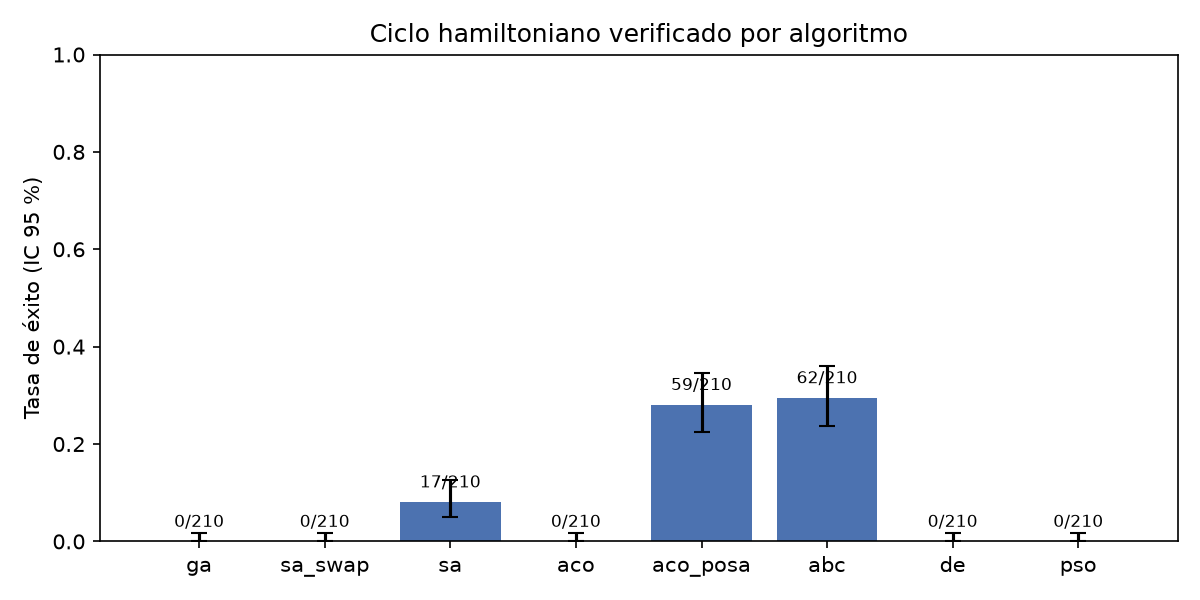
\includegraphics[width=.8\textwidth]{disenoA/exito_algoritmos.png}
\caption{Experimento A: tasa de éxito por algoritmo, con su intervalo de confianza del 95\,\%.}
\label{fig:exitoA}
\end{figure}

En cuanto al tiempo (figura~\ref{fig:tiempoA}), cuando encuentran el ciclo, \alg{ACO + Pósa}
lo hace en 1.2 segundos en la mediana y \alg{ABC} en 3.3 segundos; tres de cada cuatro éxitos
llegan antes de los 15 segundos. \alg{SA (mixto)} es más lento: tarda unos 19 segundos en la
mediana y necesita millones de evaluaciones (unos 2.7 millones) porque pasa la primera parte de la
búsqueda con la temperatura alta.

Como explicamos en la sección~\ref{sec:aco}, el número de evaluaciones de \alg{ACO + Pósa}
(unas 2\,000 en la mediana) no se puede comparar con el de los demás, porque las rotaciones de
Pósa hacen mucho trabajo que no se cuenta como evaluación.

\begin{figure}[H]
\centering
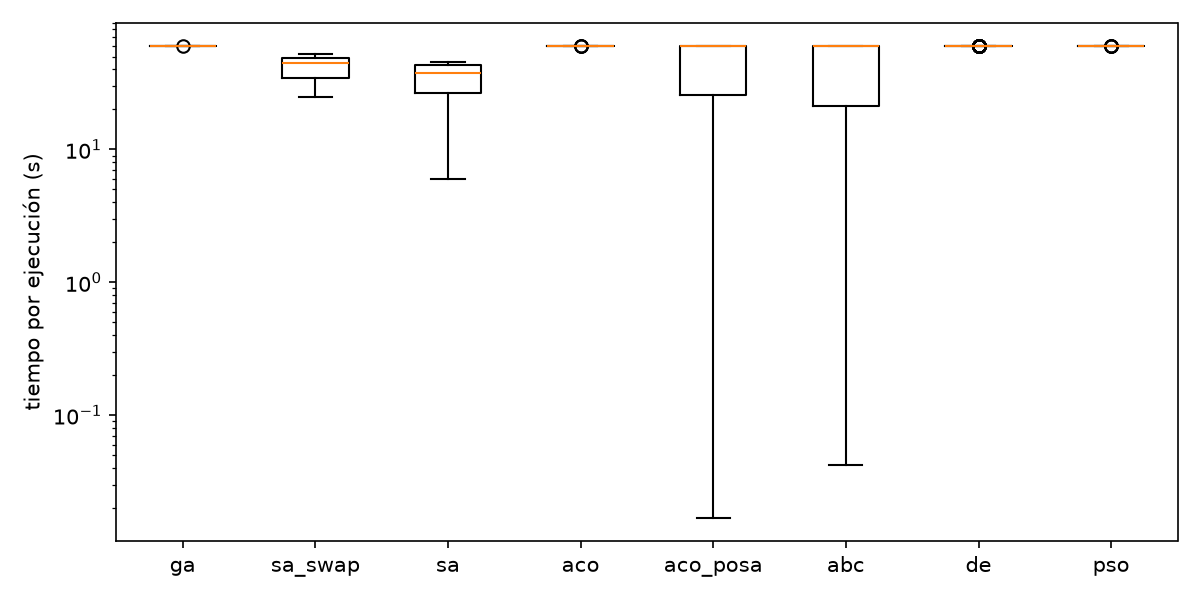
\includegraphics[width=.8\textwidth]{disenoA/tiempo_boxplot.png}
\caption{Experimento A: tiempo de cada corrida (en escala logarítmica).}
\label{fig:tiempoA}
\end{figure}

\section{Resultados por grafo}
Al ver los resultados grafo por grafo (tabla~\ref{tab:instanciasA} y figura~\ref{fig:heatmapA})
se nota que el éxito depende sobre todo del grafo. Cuando \alg{ABC} o \alg{ACO + Pósa} pueden
resolver un grafo, casi siempre lo hacen en las 10 semillas. Y hay 14 de los 21 grafos que ningún
algoritmo pudo resolver ni una vez.

\begin{table}[H]
\centering\small\filas
\caption{Experimento A: corridas exitosas (de 10) por grafo y algoritmo.}
\label{tab:instanciasA}
\resizebox{\textwidth}{!}{% Generado por Reporte/actualizar.py; no editar a mano.
\begin{tabular}{lrrcccccccc}
\toprule
Grafo & $n$ & $m$ & GA & SA (swap) & SA (mixto) & ACO & ACO + Pósa & ABC & DE & PSO \\
\midrule
graph4 & 84 & 127 & 0/10 & 0/10 & 0/10 & 0/10 & \textbf{10/10} & \textbf{9/10} & 0/10 & 0/10 \\
graph5 & 90 & 135 & 0/10 & 0/10 & 0/10 & 0/10 & 0/10 & 0/10 & 0/10 & 0/10 \\
graph6 & 94 & 142 & 0/10 & 0/10 & \textbf{6/10} & 0/10 & \textbf{10/10} & \textbf{10/10} & 0/10 & 0/10 \\
graph7 & 102 & 153 & 0/10 & 0/10 & 0/10 & 0/10 & 0/10 & 0/10 & 0/10 & 0/10 \\
graph8 & 108 & 163 & 0/10 & 0/10 & 0/10 & 0/10 & \textbf{1/10} & \textbf{3/10} & 0/10 & 0/10 \\
graph9 & 114 & 171 & 0/10 & 0/10 & 0/10 & 0/10 & 0/10 & 0/10 & 0/10 & 0/10 \\
graph10 & 118 & 178 & 0/10 & 0/10 & \textbf{4/10} & 0/10 & \textbf{10/10} & \textbf{10/10} & 0/10 & 0/10 \\
graph11 & 126 & 189 & 0/10 & 0/10 & 0/10 & 0/10 & 0/10 & 0/10 & 0/10 & 0/10 \\
graph12 & 132 & 199 & 0/10 & 0/10 & 0/10 & 0/10 & 0/10 & 0/10 & 0/10 & 0/10 \\
graph13 & 138 & 207 & 0/10 & 0/10 & 0/10 & 0/10 & 0/10 & 0/10 & 0/10 & 0/10 \\
graph14 & 142 & 214 & 0/10 & 0/10 & \textbf{3/10} & 0/10 & \textbf{10/10} & \textbf{10/10} & 0/10 & 0/10 \\
graph15 & 150 & 225 & 0/10 & 0/10 & 0/10 & 0/10 & 0/10 & 0/10 & 0/10 & 0/10 \\
graph16 & 156 & 235 & 0/10 & 0/10 & 0/10 & 0/10 & 0/10 & 0/10 & 0/10 & 0/10 \\
graph17 & 162 & 243 & 0/10 & 0/10 & 0/10 & 0/10 & 0/10 & 0/10 & 0/10 & 0/10 \\
graph18 & 166 & 250 & 0/10 & 0/10 & \textbf{3/10} & 0/10 & \textbf{10/10} & \textbf{10/10} & 0/10 & 0/10 \\
graph19 & 170 & 390 & 0/10 & 0/10 & 0/10 & 0/10 & 0/10 & 0/10 & 0/10 & 0/10 \\
graph20 & 174 & 261 & 0/10 & 0/10 & 0/10 & 0/10 & 0/10 & 0/10 & 0/10 & 0/10 \\
graph21 & 180 & 271 & 0/10 & 0/10 & 0/10 & 0/10 & 0/10 & 0/10 & 0/10 & 0/10 \\
graph22 & 186 & 279 & 0/10 & 0/10 & 0/10 & 0/10 & 0/10 & 0/10 & 0/10 & 0/10 \\
graph23 & 190 & 286 & 0/10 & 0/10 & \textbf{1/10} & 0/10 & \textbf{8/10} & \textbf{10/10} & 0/10 & 0/10 \\
graph24 & 198 & 297 & 0/10 & 0/10 & 0/10 & 0/10 & 0/10 & 0/10 & 0/10 & 0/10 \\
\bottomrule
\end{tabular}
}
\end{table}

\begin{figure}[H]
\centering
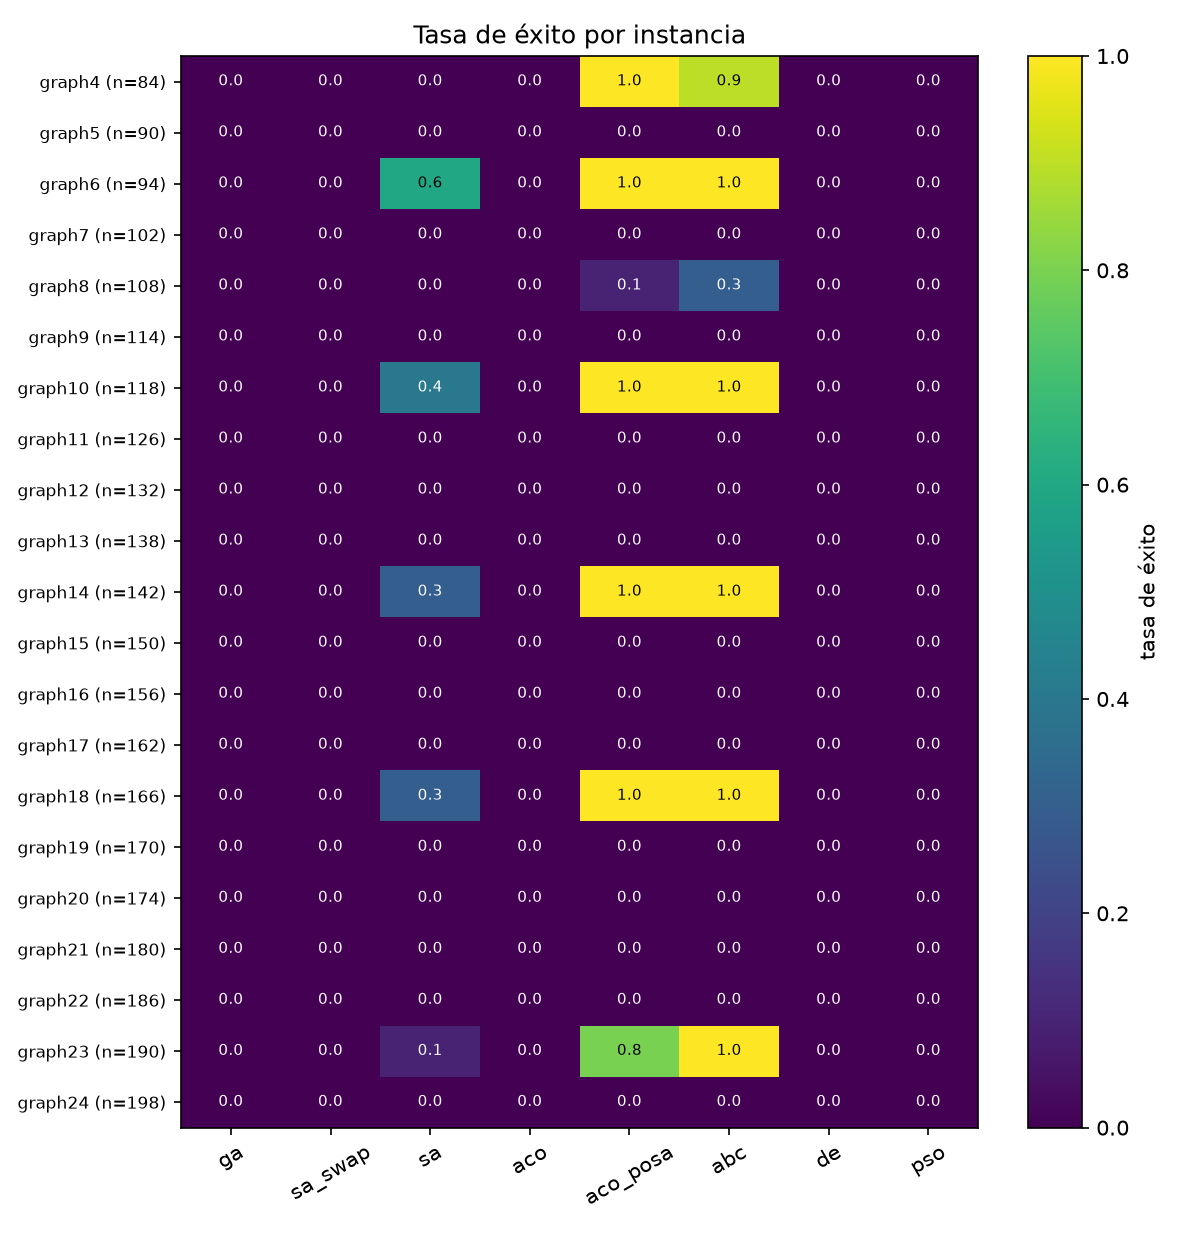
\includegraphics[width=.7\textwidth]{disenoA/heatmap_exito.png}
\caption{Experimento A: tasa de éxito por grafo y algoritmo.}
\label{fig:heatmapA}
\end{figure}

\subsection{Los grafos cúbicos}
Nos preguntamos qué tenían de especial los grafos que nadie resolvió, y al revisar los grados
encontramos un patrón muy claro. Muchos grafos del FHCP son \textbf{cúbicos}: todos sus
vértices tienen exactamente 3 vecinos. Ninguno de los 10 grafos cúbicos del experimento A se
resolvió, y en el experimento B solo se resolvió 1 de 42 (tabla~\ref{tab:cubicos}). En cambio,
los grafos que tienen algunos vértices de grado 4 se resolvieron con mucha más frecuencia.

\begin{table}[H]
\centering\filas
\caption{Grafos resueltos (por cualquier algoritmo) según si son cúbicos o no.}
\label{tab:cubicos}
% Generado por Reporte/actualizar.py; no editar a mano.
\begin{tabular}{lcc}
\toprule
Experimento & Grafos cúbicos resueltos & Grafos no cúbicos resueltos \\
\midrule
A (graph4--graph24) & 0 de 10 & 7 de 11 \\
B (graph1--graph100) & 1 de 42 & 19 de 58 \\
\bottomrule
\end{tabular}

\end{table}

Tiene sentido: con solo 3 vecinos por vértice hay muy pocas formas de entrar y salir de cada uno,
así que casi cualquier decisión equivocada deja a algún vértice sin salida. Esto concuerda con
la idea del FHCP de reunir grafos con estructuras pensadas para ser difíciles \cite{aco8}.

\section{Cómo mejora cada algoritmo (convergencia)}
Las gráficas de convergencia muestran cómo baja el número de aristas faltantes conforme el
algoritmo hace más evaluaciones (figuras~\ref{fig:convA14} y~\ref{fig:convA}). Cada línea es la
mediana de las 10 semillas.

\begin{figure}[H]
\centering
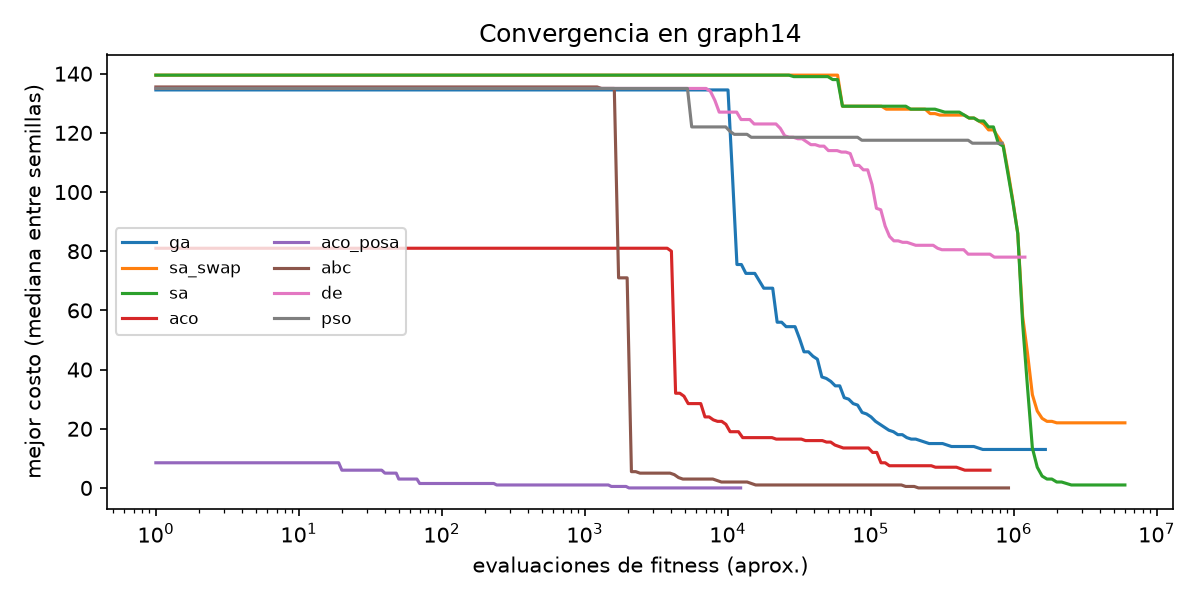
\includegraphics[width=\textwidth]{disenoA/convergencia_graph14.png}
\caption{Experimento A: convergencia en graph14 (142 vértices).}
\label{fig:convA14}
\end{figure}

\begin{figure}[H]
\centering
\begin{subfigure}{.49\textwidth}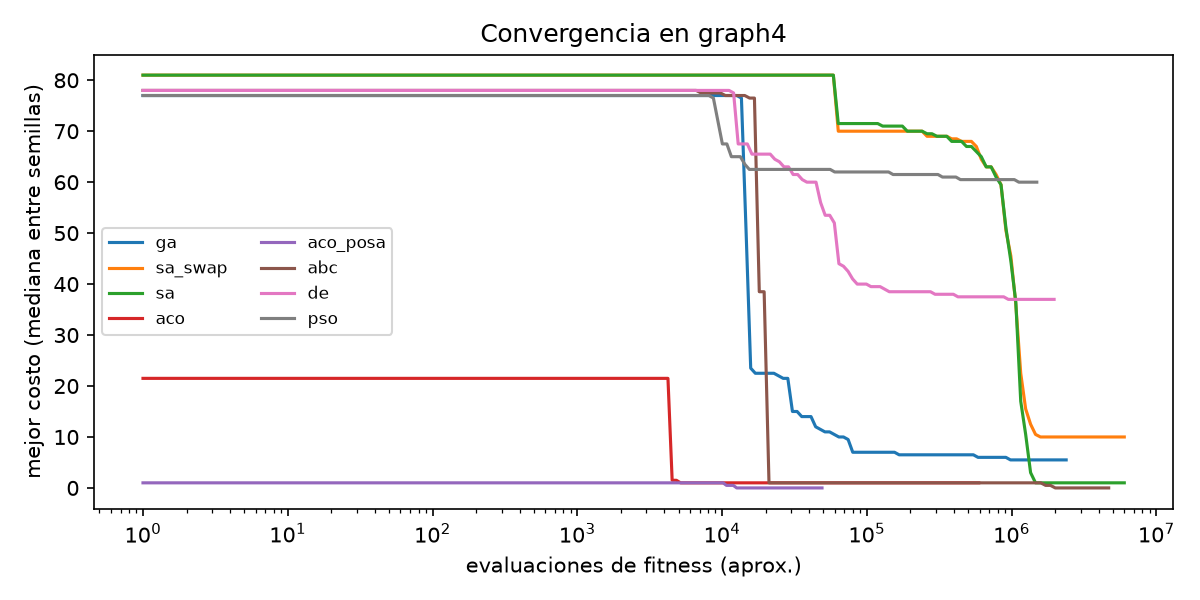
\includegraphics[width=\textwidth]{disenoA/convergencia_graph4.png}\caption{graph4 (84 vértices)}\end{subfigure}
\begin{subfigure}{.49\textwidth}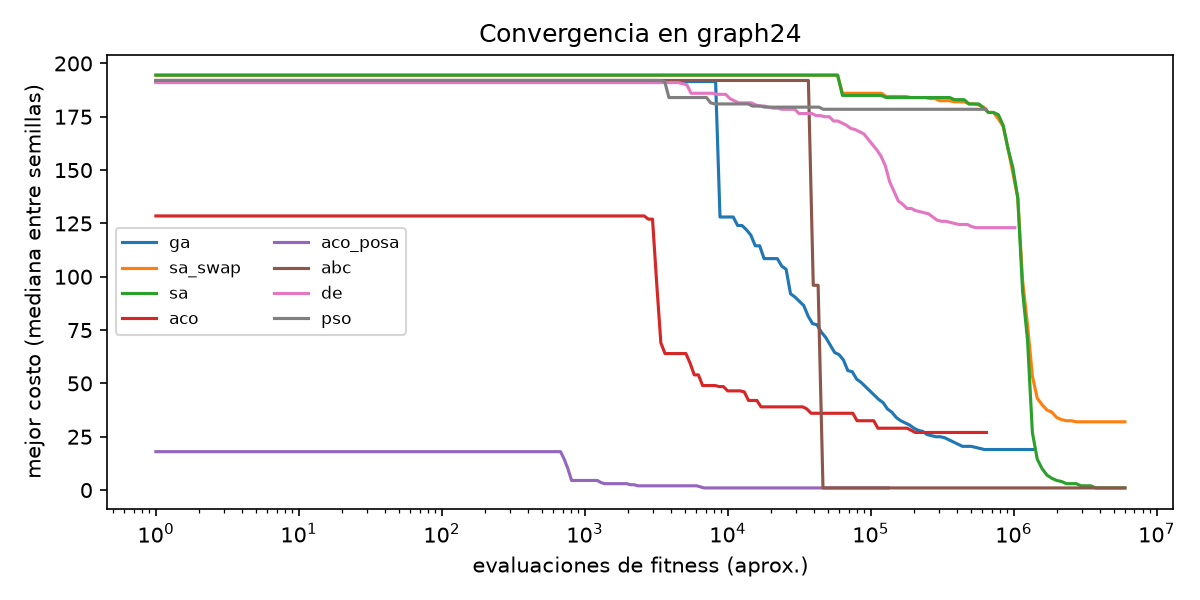
\includegraphics[width=\textwidth]{disenoA/convergencia_graph24.png}\caption{graph24 (198 vértices)}\end{subfigure}
\caption{Experimento A: convergencia en el grafo más pequeño y en el más grande.}
\label{fig:convA}
\end{figure}

Lo que observamos:
\begin{itemize}
  \item \alg{ACO + Pósa} empieza ya muy cerca de la solución, porque las hormigas construyen las
        rutas sobre aristas reales y las rotaciones las alargan.
  \item \alg{ABC} baja de golpe en las primeras miles de evaluaciones, gracias a la inversión
        guiada, y luego afina poco a poco.
  \item \alg{SA} casi no mejora al principio, porque con la temperatura alta acepta muchos cambios
        malos. Ya que se enfría, baja muy rápido y llega cerca de cero, pero tarde.
  \item \alg{GA} y \alg{ACO} sin rotaciones mejoran al principio y luego se estancan.
  \item \alg{DE} y \alg{PSO} apenas mejoran y se quedan con muchas aristas faltantes. Con
        \emph{random keys}, un cambio pequeño en los números puede reordenar media ruta, así que
        al algoritmo le cuesta mucho ir mejorando poco a poco.
\end{itemize}

\section{Qué tan cerca se quedaron}
La figura~\ref{fig:costoA} muestra las aristas faltantes al terminar. Aunque no encontraran el
ciclo, \alg{ABC}, \alg{ACO + Pósa} y \alg{SA (mixto)} se quedaron en promedio a menos de una
arista de la solución. \alg{DE} y \alg{PSO} quedaron muy lejos (79 y 119 aristas faltantes en
promedio).

\begin{figure}[H]
\centering
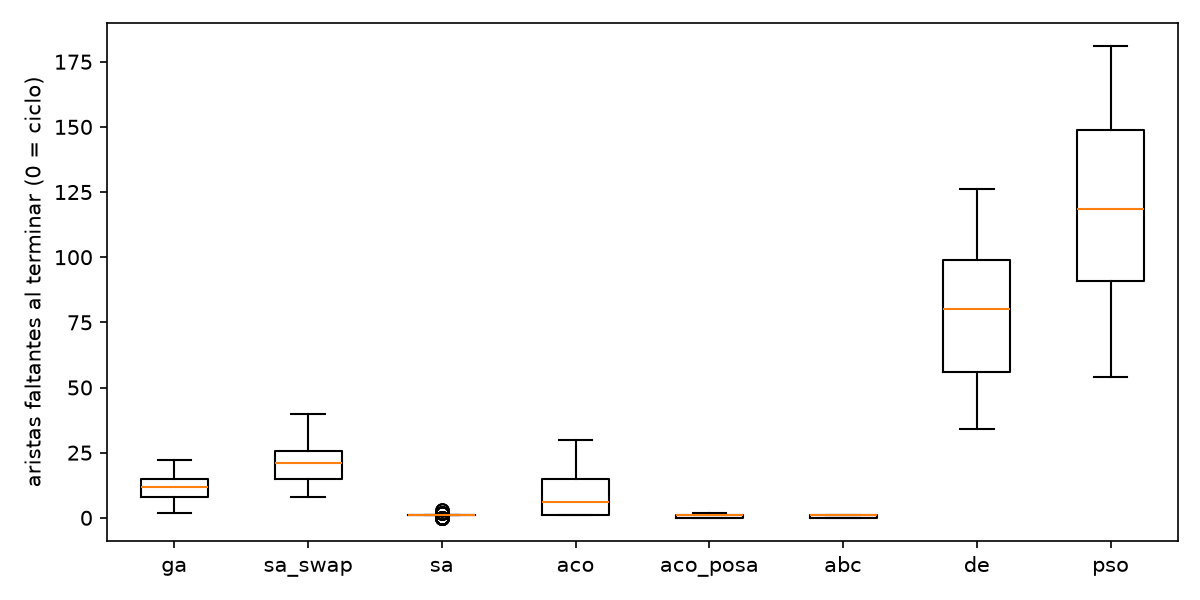
\includegraphics[width=.8\textwidth]{disenoA/costo_final_boxplot.png}
\caption{Experimento A: aristas faltantes al terminar (0 significa que encontró el ciclo).}
\label{fig:costoA}
\end{figure}

\section{Grafos grandes (experimento C)}
En el experimento C probamos los ocho algoritmos con grafos mucho más grandes, con un límite de
2 minutos (tabla~\ref{tab:escalabilidad}). Ninguno encontró un ciclo, pero la diferencia en qué
tan cerca quedaron es enorme. En graph1001, con 9\,528 vértices, a \alg{ABC} le faltaron solo 88
aristas; a \alg{SA (mixto)}, más de 9\,000, y \alg{DE} y \alg{PSO} quedaron prácticamente igual que
una ruta al azar. En graph50 (348 vértices), a \alg{ABC} y a \alg{SA (mixto)} les faltó
\emph{una sola arista}.

\begin{table}[H]
\centering\small\filas
\caption{Experimento C: aristas faltantes al terminar. En negritas, el mejor resultado de cada grafo (una semilla, \tiempoC\,s).}
\label{tab:escalabilidad}
\resizebox{\textwidth}{!}{% Generado por Reporte/actualizar.py; no editar a mano.
\begin{tabular}{lrrrrrrrrrr}
\toprule
Grafo & $n$ & $m$ & GA & SA (swap) & SA (mixto) & ACO & ACO + Pósa & ABC & DE & PSO \\
\midrule
graph50 & 348 & 523 & 35 & 51 & \textbf{1} & 97 & 7 & \textbf{1} & 253 & 323 \\
graph200 & 1200 & 1902 & 649 & 284 & 76 & 579 & 369 & \textbf{9} & 1167 & 1182 \\
graph500 & 2915 & 7271 & 2385 & 995 & 585 & 2549 & 1462 & \textbf{21} & 2889 & 2897 \\
graph1001 & 9528 & 13968 & 9436 & 5806 & 9087 & 8806 & 7201 & \textbf{88} & 9515 & 9516 \\
\bottomrule
\end{tabular}
}
\end{table}

\begin{figure}[H]
\centering
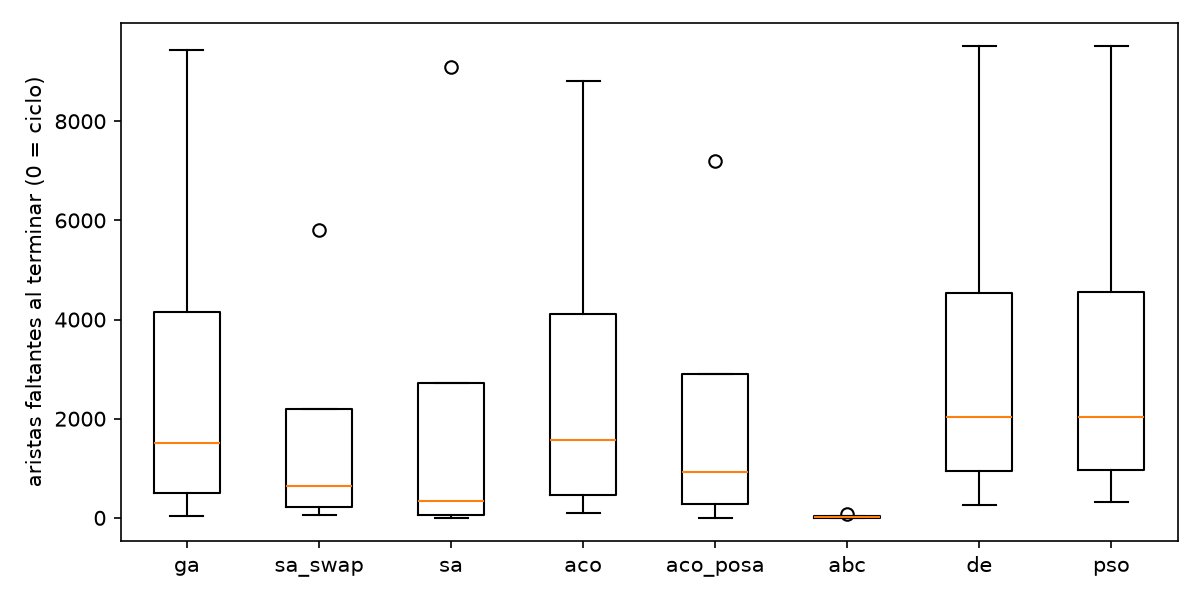
\includegraphics[width=.8\textwidth]{disenoC/costo_final_boxplot.png}
\caption{Experimento C: aristas faltantes al terminar.}
\label{fig:costoC}
\end{figure}

Si vemos las aristas faltantes como porcentaje del total de vértices, \alg{ABC} se mantiene por
debajo del 1\,\% incluso en el grafo más grande, mientras que los demás algoritmos empeoran
mucho conforme crece el grafo. Es decir, \alg{ABC} es el único que escala razonablemente bien.
